\documentclass[12pt, letterpaper, twoside]{article}
\usepackage[sorting=none, backend=bibtex]{biblatex} %Imports biblatex package
\bibliography{ref} %Import the bibliography file
\usepackage[hmarginratio=1:1]{geometry}
\usepackage[utf8]{inputenc}
\usepackage{graphicx}
\graphicspath{ {./img/} }
\usepackage{float}
\usepackage{hyperref}
\usepackage{subcaption}
\usepackage{wrapfig}
\usepackage[inline]{enumitem}

\title{Neural Network Project - MobileNet v3}
\author{Salvatore Cognetta 1874383}
        
\date{January 2022}

\begin{document}

\begin{titlepage}
\maketitle
\end{titlepage}

\clearpage
\thispagestyle{empty}
\vspace*{\fill}
MobileNetV3 implementation for Neural Network course project, Artificial Intelligence and Robotics, Sapienza.
\vspace*{\fill}
\clearpage


\tableofcontents

\clearpage
    
\clearpage
\section{Introduction}
Nell'ultimo decennio la potenza di device portatili di piccole dimensioni, come gli smartphone, è cresciuta in modo esponenziale, quasi a raggiungere potenze di low-budget computer. Questo ha fatto sì che si studiasse la possibilità di utilizzo di reti neurali su questi devices. \\
Come sappiamo, utilizzare tecniche di machine learning è molto heavy load, per tale motivo è necessario fare delle assumptions prima di addentrarsi in questo modo. Allo stato attuale è impensabile effettuare il train su un singolo device mobile con così poca potenza wrt workstation e big datacenter utilizzate generalmente per il train delle reti. Anche se l'edge computing e la possibilità di utilizzare un'insieme di devices contemporaneamente anche per il train di reti neurali si fa sempre più insistente, in questo lavoro ci focalizziamo su un altro tipo di studio: nello specifico nell'utilizzo di lightweight reti neurali, appositamente ingegnerizzate, che vengono trainate a priori ma che possono essere utilizzate per fare inference proprio sui device mobili, come gli smartphone. \\
In questo senso, abbiamo deciso di implementare quella che è allo stato attuale la state of the art per questo tipo di reti e cioè MobileNetV3 \cite{howard2019searching}. Gli autori propongono due tipologie di reti, che vengono chiamate MobileNetV3 Small and Large. La prima si è un'evoluzione della rete MobileNetV2 \cite{sandler2019mobilenetv2}, mentre la seconda si basa sul lavoro contenuto in MnasNet-A1 \cite{tan2019mnasnet}. \\

The goal of the reference paper is to develop the best possible mobile computer vision architectures optimizing the accuracy-latency trade off on mobile devices. To accomplish this they introduce (1) complementary search techniques, (2) new efficient versions of nonlinearities practical for the mobile setting, (3) new efficient network design, (4) a new efficient segmentation decoder.\\
In questo lavoro viene implementata la soluzione proposta in MobileNetV3 e applicata a due dataset differenti per image detection and classification: MNIST \cite{deng2012mnist} and CIFAR10 \cite{Krizhevsky09learningmultiple}.

\section{Related works}
Tale lavoro, come già detto, è un evoluzione di MobileNetV2 alla ricerca di un modello quasi-ottimo per soluzioni con poca potenza computazionale. Per realizzare questa soluzione è ovviamente necessario raggiungere un punto di trade-off tra l'accuratezza del modello e la complessità computazionale in fase di inferenza (efficienza). Both novel handcrafted structures and algorithmic neural architecture search have played important roles in advancing this field.\\

For example, as stated by the authors, in SqueezeNet \cite{iandola2016squeezenet} 1x1 convolutions with squeeze and expand modules are extensively used, primarily focusing on reducing the number of parameters. More recent works shifts the focus from reducing parameters to reducing the number of operations (MAdds) and the actual measured latency. \\ 
MobileNetV1 \cite{howard2017mobilenets} employs depthwise separable convolution to substantially improve computation efficiency; while MobileNetV2 \cite{sandler2019mobilenetv2} expands on this by introducing a resource-efficient block with inverted residuals and linear bottlenecks. \\
More studies on the subject, like ShuffleNet \cite{zhang2017shufflenet}, CondenseNet \cite{huang2018condensenet} and ShiftNet \cite{yan2018shiftnet} were taken into account by the authors for the uses of group convolution at training phase and shift operation with point-wise convolutions in order to replace expensive spatial convolutions. \\

Another major study performed regards the automatization of the architecture design search, which can be done using Reinforcement Learning to search efficient architectures with interesting and very good accuracy.\\
Recently, the authors in MnasNet \cite{tan2019mnasnet} explored a block-level hierarchical search space allowing different layer structures at different resolution blocks of a network.\\

\clearpage
\section{Solutions}
All these above mentioned ideas and studies are taken into account by the authors and used, together with other innovative proposal, reaching state of the art network for mobile devices, as explained in this section.

\subsection{MobileNetV3 Block}
block

\subsection{Network search}
block

\subsection{Nonlinearities}
As a replacement for the ReLU function, the swish nonlinearity is taken into account. It can be defined as 
$$swish(x) = x \cdot \sigma(x)$$
This nonlinearities improves the overall accuracy, however it's more expensive because of the sigmoid function, difficult to compute on mobile devices. \\
For this reason it's replaced with its piece-wise linear hard analog:
$$hswish(x) = x \frac{ReLU6(x+3)}{6}$$

This hard version have no big differeces in terms of accuracy. A comparison beetwen them can be seen in figure \ref{fig:hswish_comparison}

\begin{figure}[h]
	\centering
	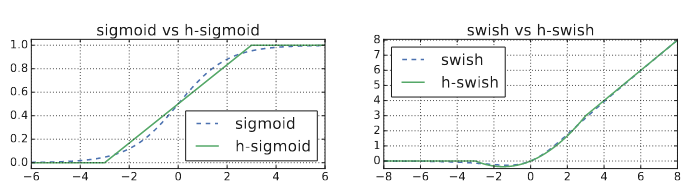
\includegraphics[width=1\textwidth]{hswish}
	\caption{Comparision between Sigmoid and swish function with their hard corrispective}
	\label{fig:hswish_comparison}
\end{figure}


\clearpage
\section{Implementation}
The MobileNetV3 consists of two different design architectures, one used for high resources and another one for low resources, respectively Large and Small models. In this work both of them are implemented from scratch using pytorch and pytorch-lightning, framework used essentially to simplify multi-gpu training, using Distributed Data Parallel paradigm. \\
Initially the implementation was done using Jupyter Notebooks, however cause of a bug regarding multi-gpu training, the implementation was completed using classical python script files. \\
Both proposed model, small and large, were trained using the structure defined by the authors and replicated in the Figure~\ref{fig:specifications}.

\begin{figure}[h]
	\centering
	\begin{subfigure}{.5\textwidth}
		\centering
		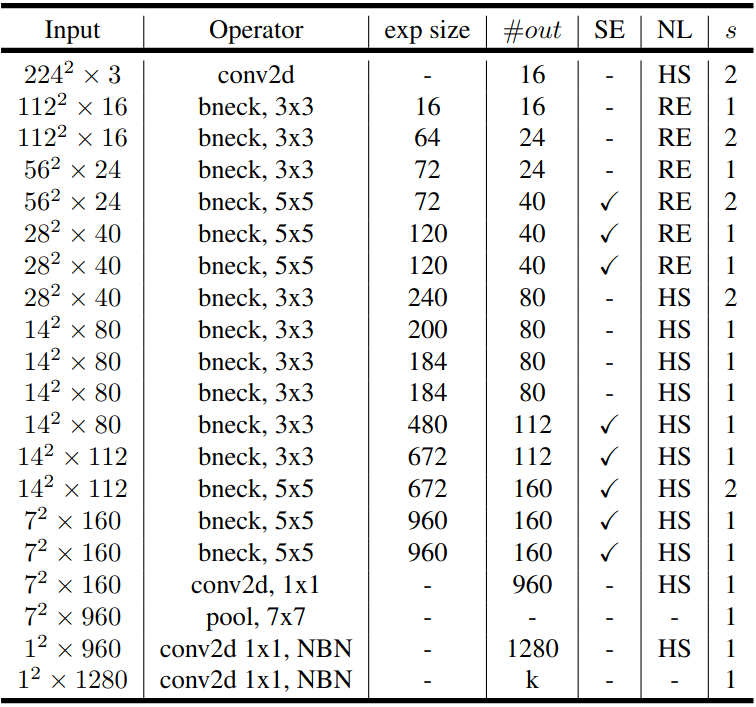
\includegraphics[width=.9\linewidth]{spec_large.png}
		\caption{Large model}
	\end{subfigure}%
	\begin{subfigure}{.5\textwidth}
		\centering
		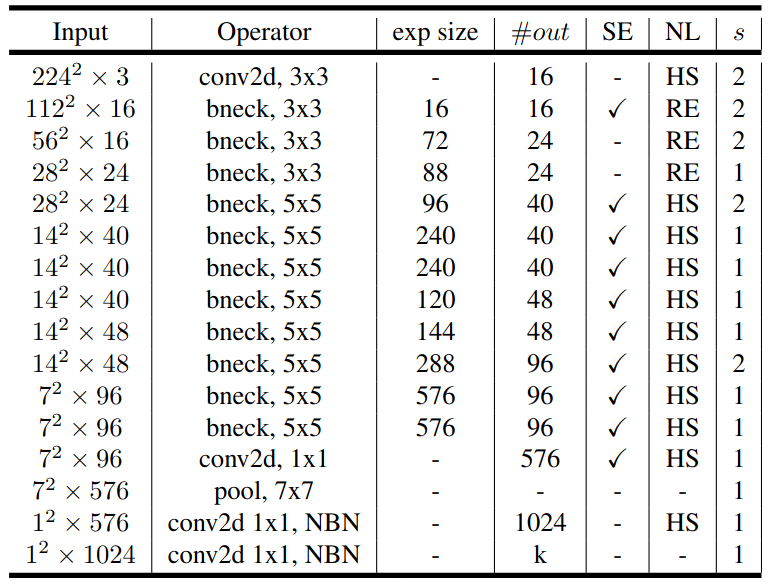
\includegraphics[width=.9\linewidth]{spec_small.png}
		\caption{Small model}
	\end{subfigure}
	\caption{MobileNetV3 specifications for Large and Small model}
	\label{fig:specifications}
\end{figure}

These specifications are stored inside two different json files, loaded before training the neural network to create the model architecture on the fly. Every row of the table \ref{fig:specifications} is associated to an object of the json file, containg:
\begin{itemize}
	\item the input and output size
	\item kernel size
	\item the stride size
	\item expansion dimension
	\item if the squeeze and excite must be used
	\item the type of non-linearity to be used (ReLU or hard-swish)
\end{itemize}

\subsection{Adroid app}
After the training all the models are transformed in order to use them in an android workspace. The workflow followed for this operation can be seen in figure \ref{fig:pytorch_mobile}, which consists in the scripting of the model with the \textit{just in time} built-in pytorch compiler and the transformation of this to a model for pytorch lite.

\begin{figure}[H]
	\centering
	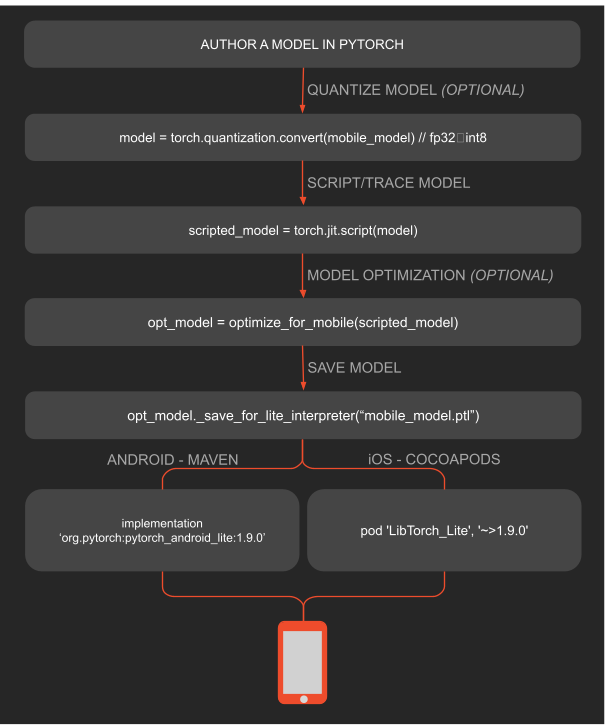
\includegraphics[width=0.6\textwidth]{pytorch-mobile.png}
	\caption{Mobile deployment workflow: https://pytorch.org/mobile/home/}
	\label{fig:pytorch_mobile}
\end{figure}

After this workflow as output we have a model that is ready to use inside a Android or iOS app. To make a demo, we created a simple app in Android Studio using Kotlin, in order to test the mobile version of the trained models.\\
The app is very simple, as shown in the figure \ref{fig:demo_app}. In the main view the image to be predicted is shown, while on the bottom the prediction is set in a light grey box. There are two buttons, always on the bottom, one for Mnist and another one for Cifar10 image prediction. Both of them upload the needed model, put inside the asset folder, while a new image is randomly chosen inside the associated asset directory (\verb|asset/MNIST| or \verb|asset/Cifar10|).

\begin{figure}[H]
	\centering
	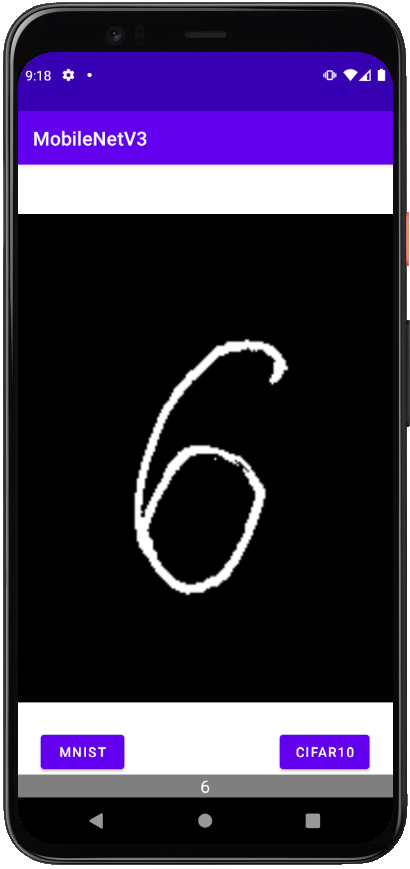
\includegraphics[width=0.4\textwidth]{demo_app.png}
	\caption{Android demo app}
	\label{fig:demo_app}
\end{figure}

Even if this is only a demo app, it's noticeable that, without using model quantization and suitable optimization, there is a significant drop in model accuracy, underlying moreover the improvements that can be done using model inference on mobile devices.

\clearpage
\section{Experiments and results}
The implementation of MobileNetV3 in this work is trained and test using two different datasets: \verb|MNIST| and \verb|Cifar10|. \\
Both of them are trained using normalization of the channels using Gaussian Normalization. Upsampling to a dimension of 224 width and 224 height is also needed for the images, considering the low quality of the networks.\\
All the datasets are splitted in training and validation set, in a classical way to evaluate the network on never seen images and trying to not occurr in overfitting.

\subsection{MNIST}
The MNIST dataset consist in a collection of black and white (one channel) images of hand written digit.\\
The classification of the MNIST dataset is a very simple task for this kind of networks, for this reason only the small version of MobileNetV3 is trained on this dataset.\\
In this case a Gaussian Normalization with mean and standard deviation in $0.5$ is firstly applied, with some data augmentation using the transforms built-in function of the torchvision framework: random crop and random horizontal flip is applied to training dataset.\\
The network is trained for 50 epochs.\\
As we can see from Figure~\ref{fig:mnist_acc} the accuracy during training reaches high values after only 10 epochs, while in Figure~\ref{fig:mnist_loss} we can notice a complementar pattern for the training loss.\\

\begin{figure}[h]
	\centering
	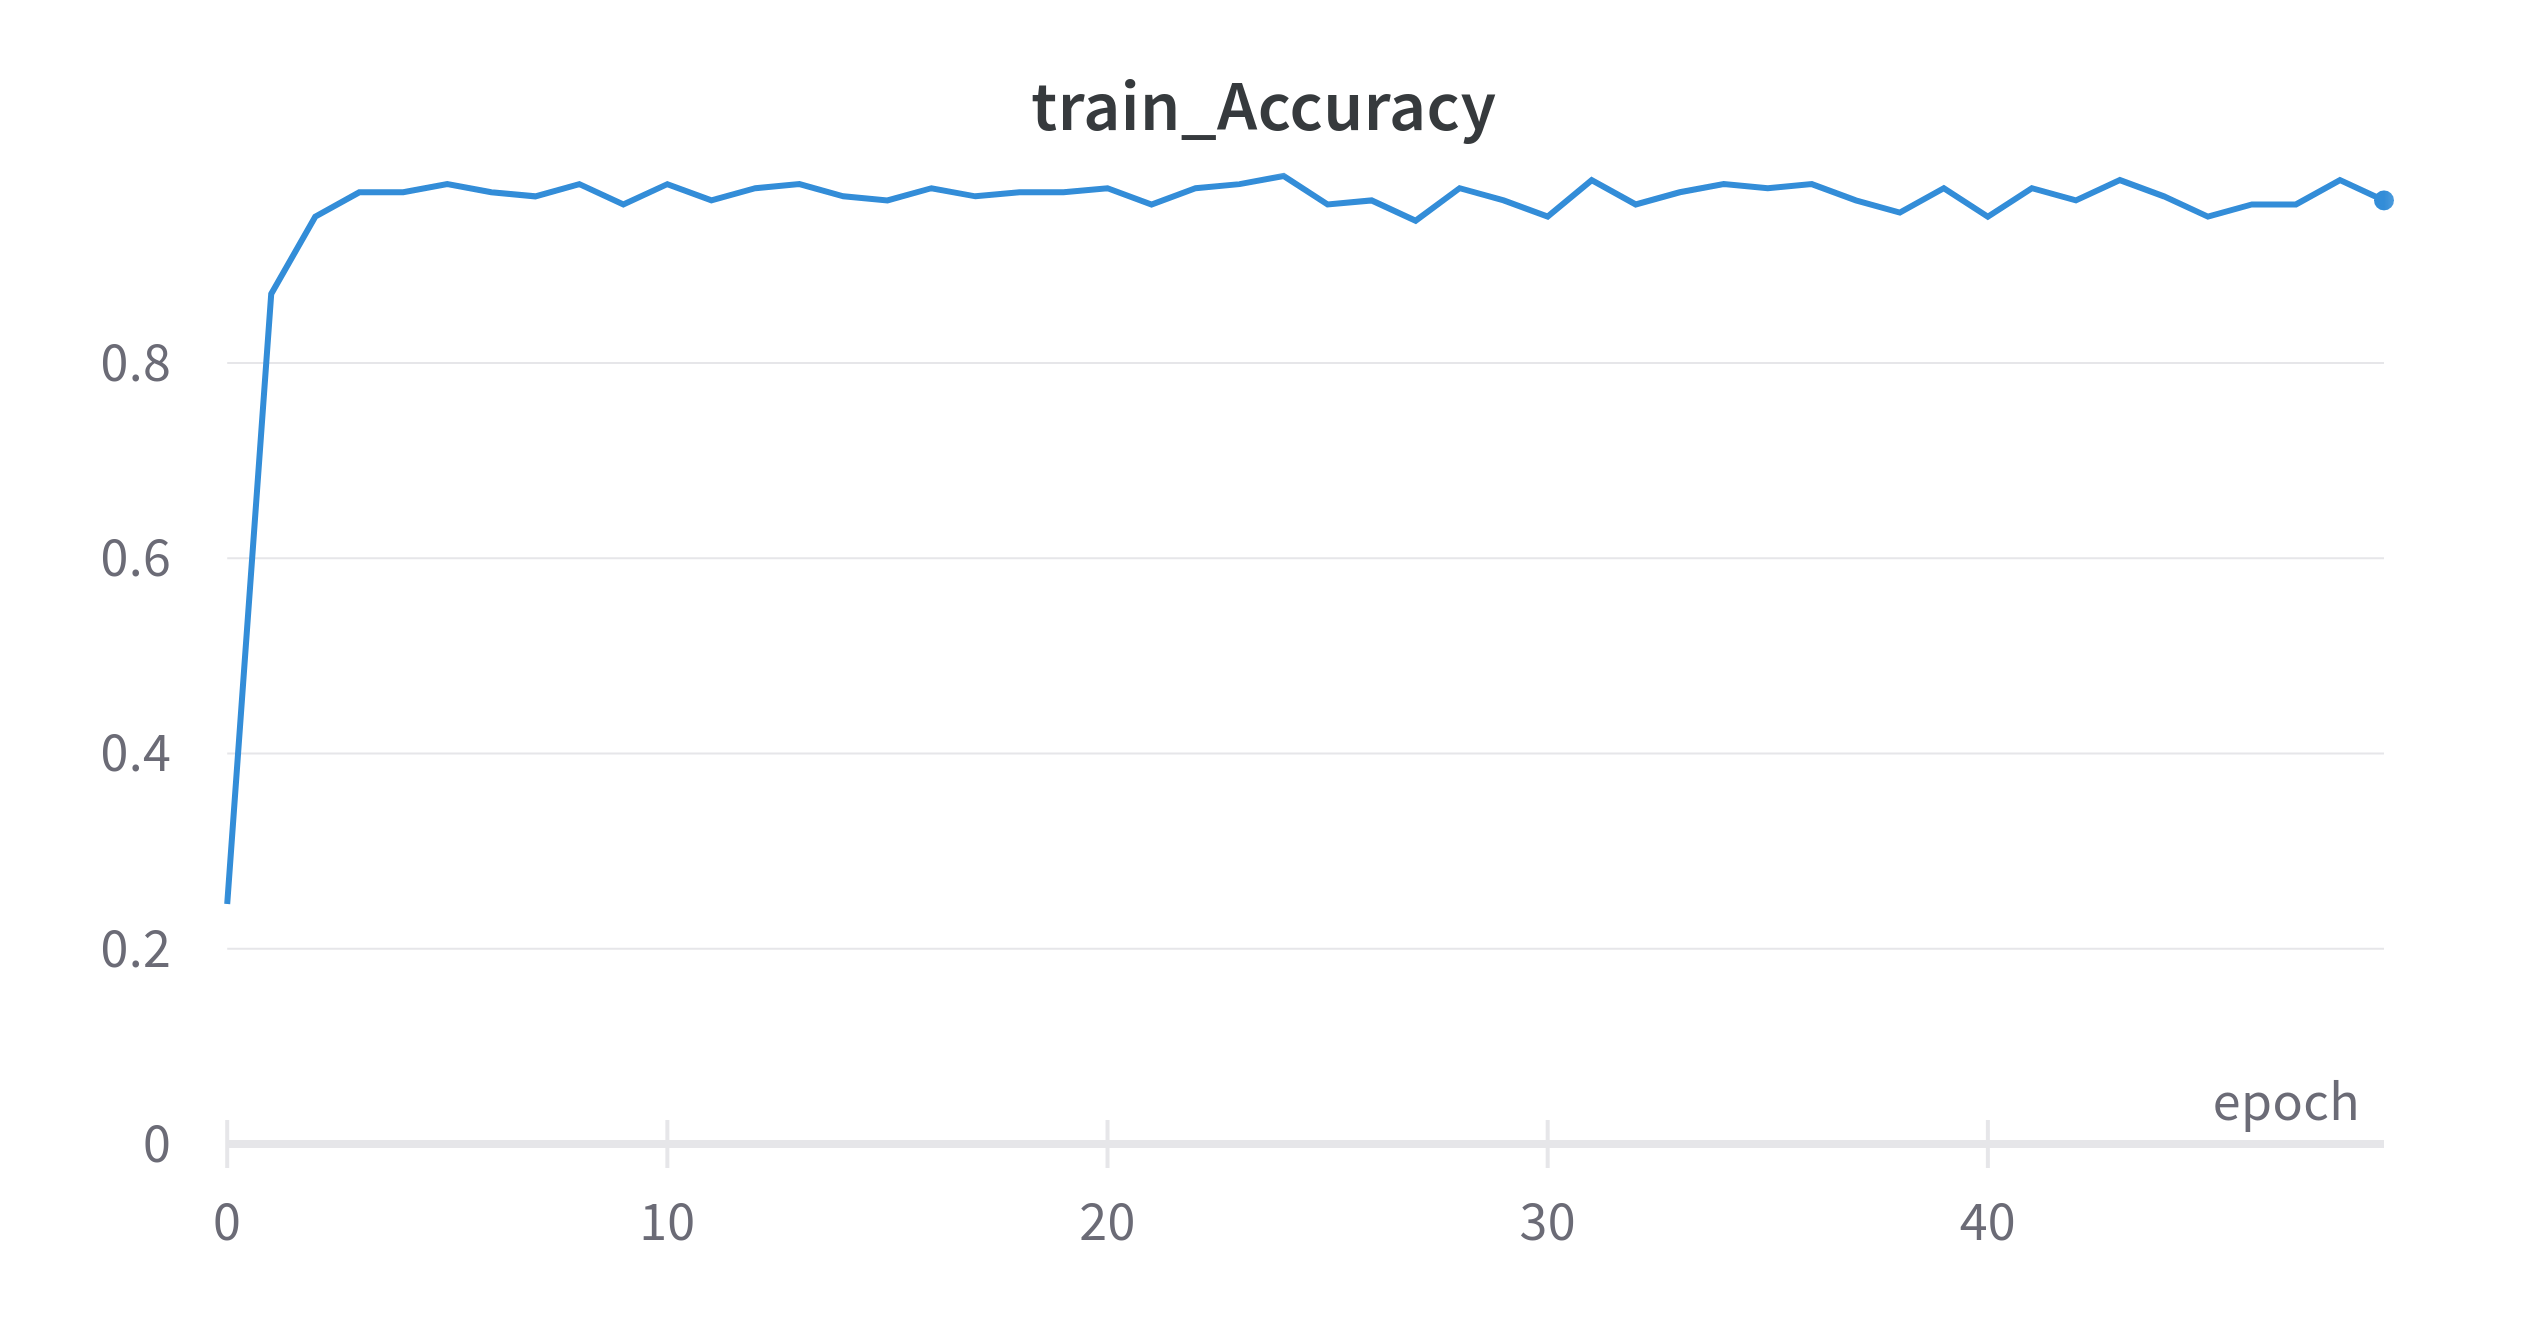
\includegraphics[width=.7\textwidth]{mnet_small_mnist_accuracy.png}
	\caption{Mnist train accuracy}
	\label{fig:mnist_acc}
\end{figure}

\begin{figure}[h]
	\centering
	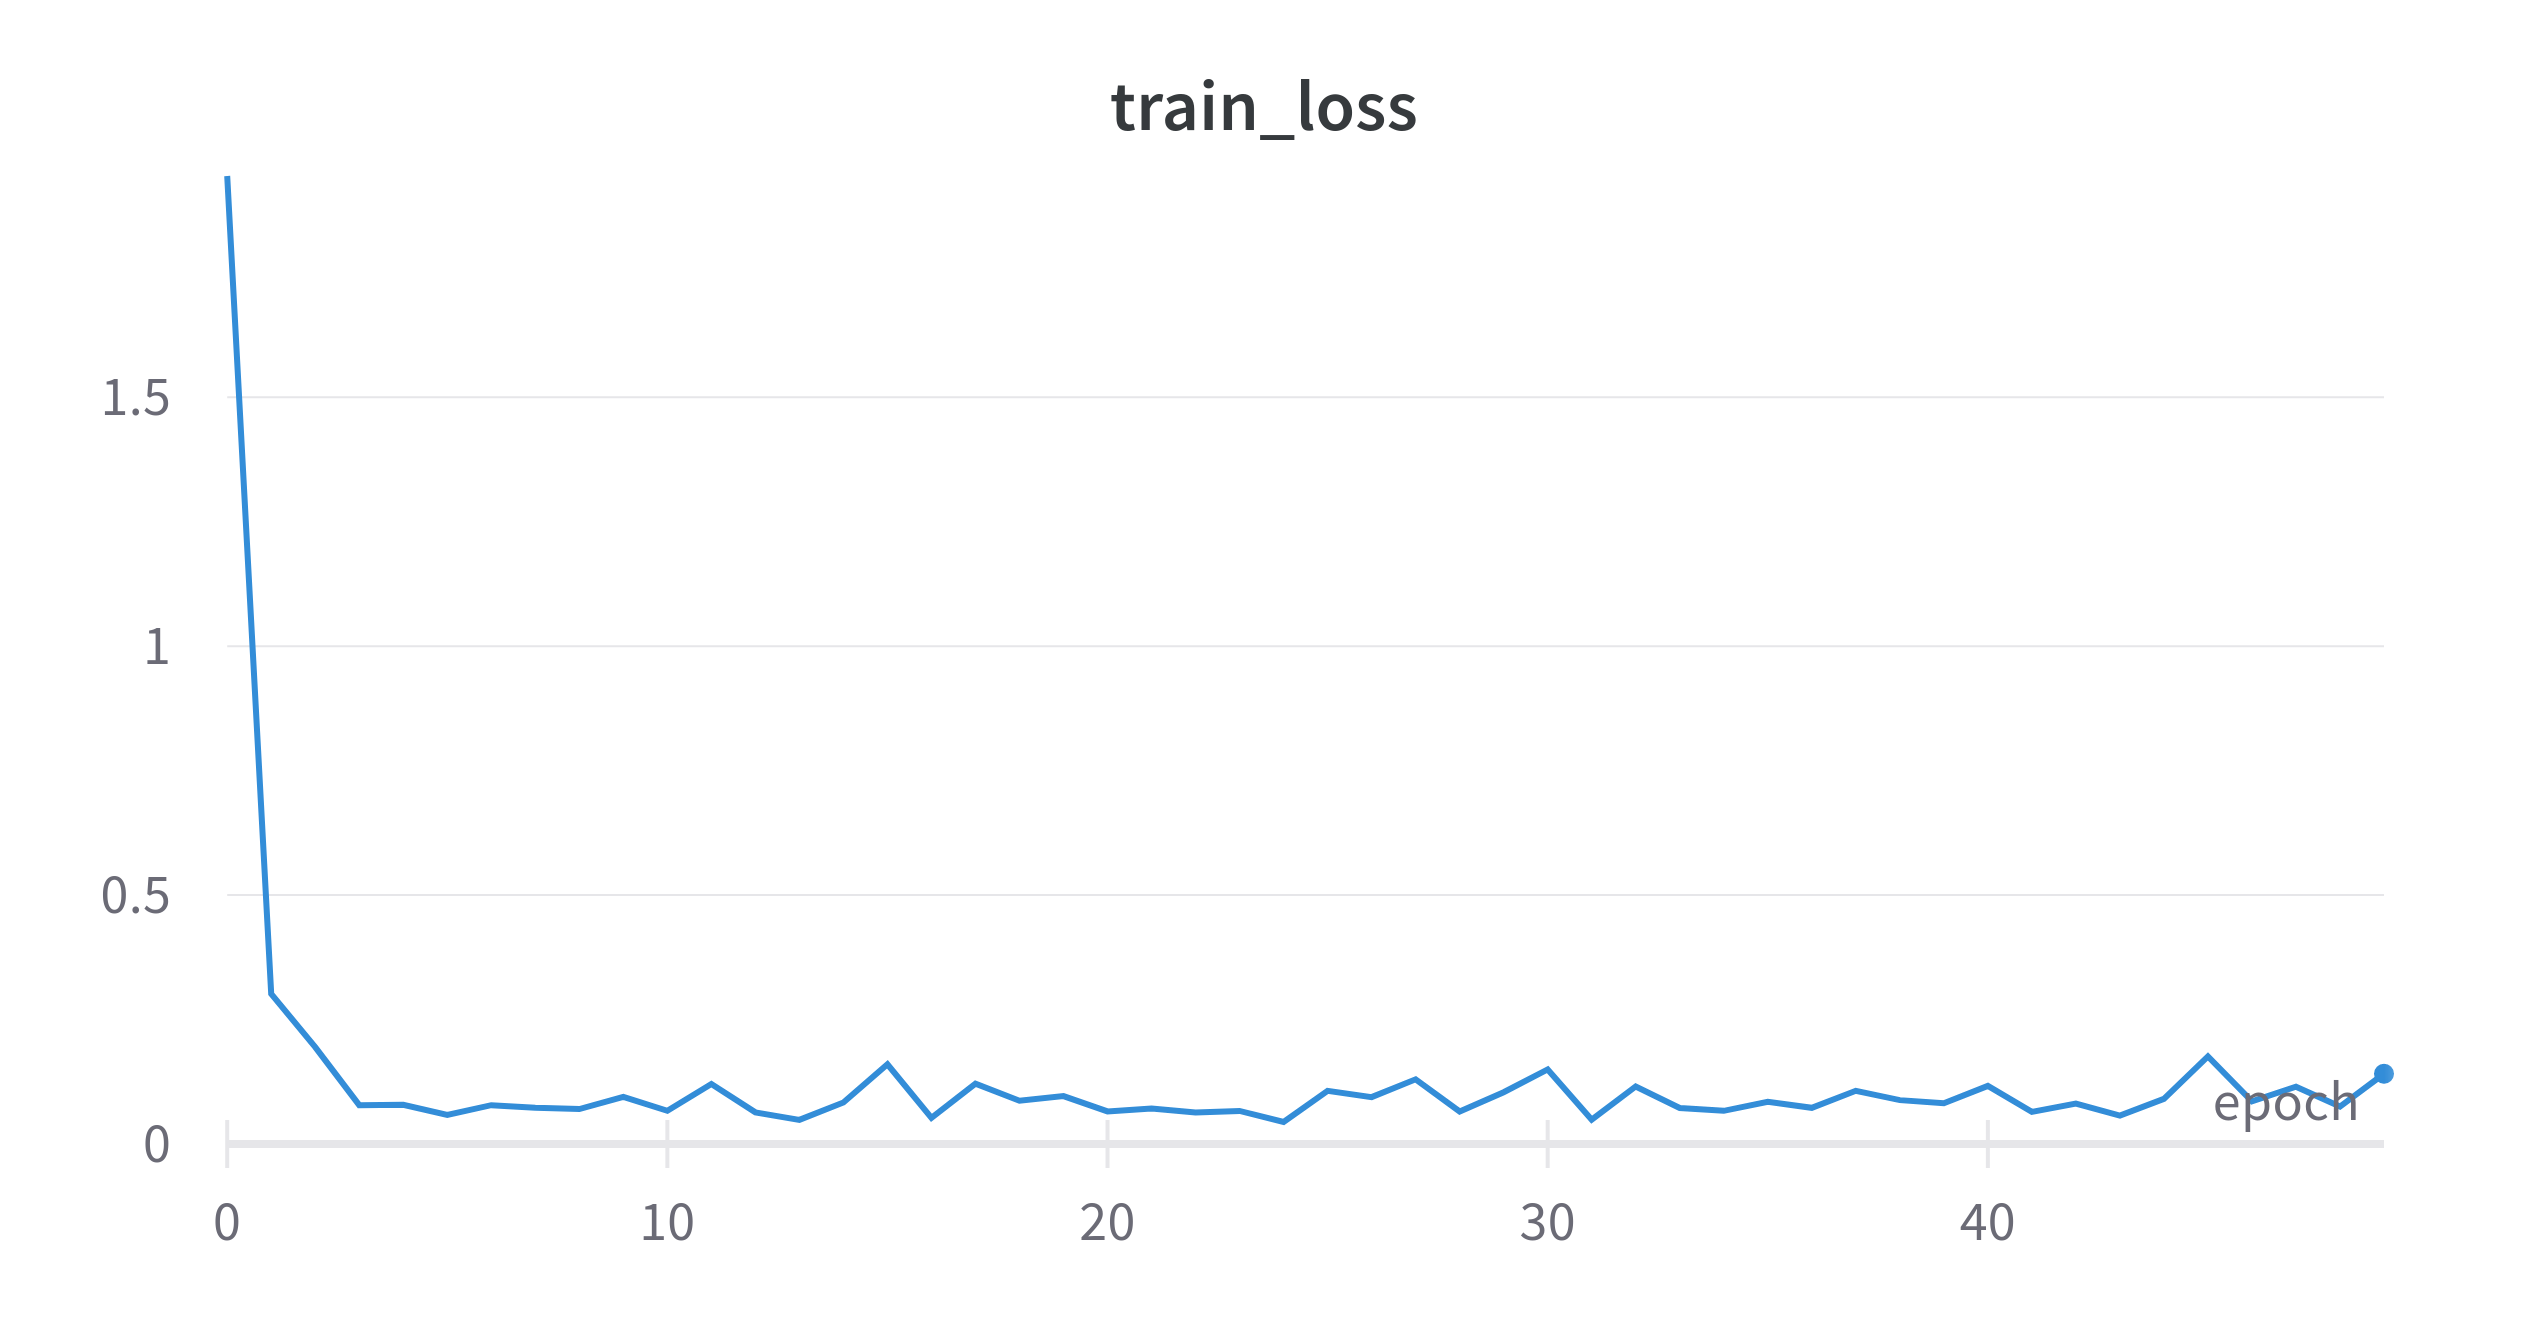
\includegraphics[width=.7\textwidth]{mnet_small_mnist_loss.png}
	\caption{Mnist train loss}
	\label{fig:mnist_loss}
\end{figure}

After training the test dataset is used for evaluation, in this case we notice an overall test accuracy very high, about $0.95\%$. The associated classification report with all the evaluation metrics is shown in Figure~\ref{fig:mnist_class_report}.\\

In the confusion matrix plotted in Figure~\ref{fig:mnist_cm} we can notice that the netwrok has an high sensitivity with the number $1$ while it struggles more with number $5$, confused often with numbers $2$ and $3$.

\begin{figure}[ht]
	\centering
	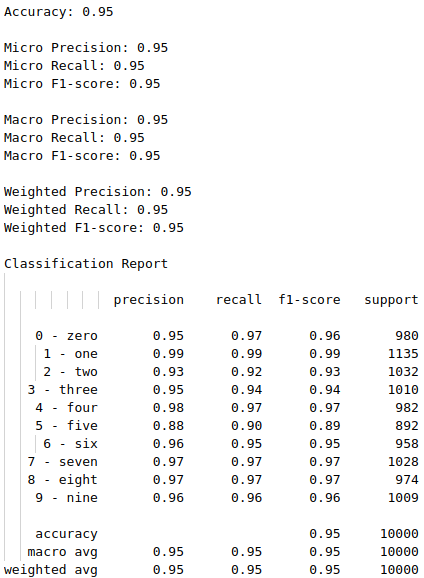
\includegraphics[width=.5\textwidth]{report_mnist_small.png}
	\caption{Mnist classification report}
	\label{fig:mnist_class_report}
\end{figure}

\begin{figure}[H]
	\centering
	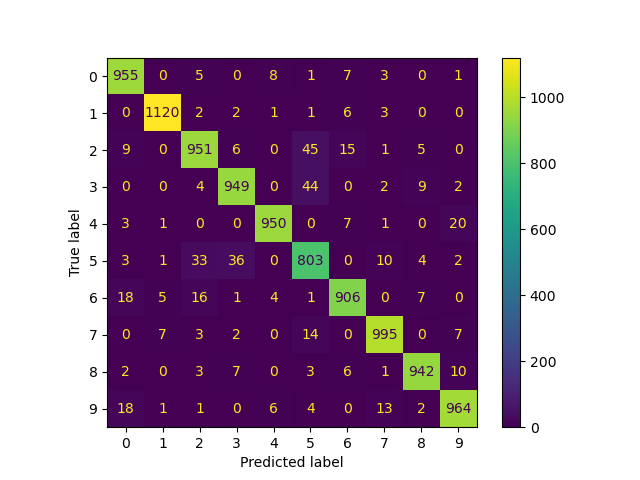
\includegraphics[width=.8\textwidth]{cm_mnist_small.png}
	\caption{Mnist confusion matrix}
	\label{fig:mnist_cm}
\end{figure}



\subsection{Cifar10}
The Cifar10 dataset consist in a collection of rgb (three channels) images belonging to 3 different categories.\\
This classification task is more complex than the MNIST one, for this reason in this work the train is done with both the networks architectures, Small and Large.\\
Also in this case a Gaussian Normalization is used with mean in $[0.485, 0.456, 0.406]$ and standard deviation in $[0.247, 0.243, 0.261]$ is firstly applied. Like before, some data augmentation is applied: random crop and random horizontal flip is applied to training dataset.\\
The network is trained for 25 epochs.\\
\paragraph{Small} 
As we can see from Figure~\ref{fig:cifar10_small_stride2_acc} the accuracy during training reaches not so good values, while in Figure~\ref{fig:cifar10_small_stride2_loss} we can notice a complementar pattern for the training loss.\\

\begin{figure}[H]
	\centering
	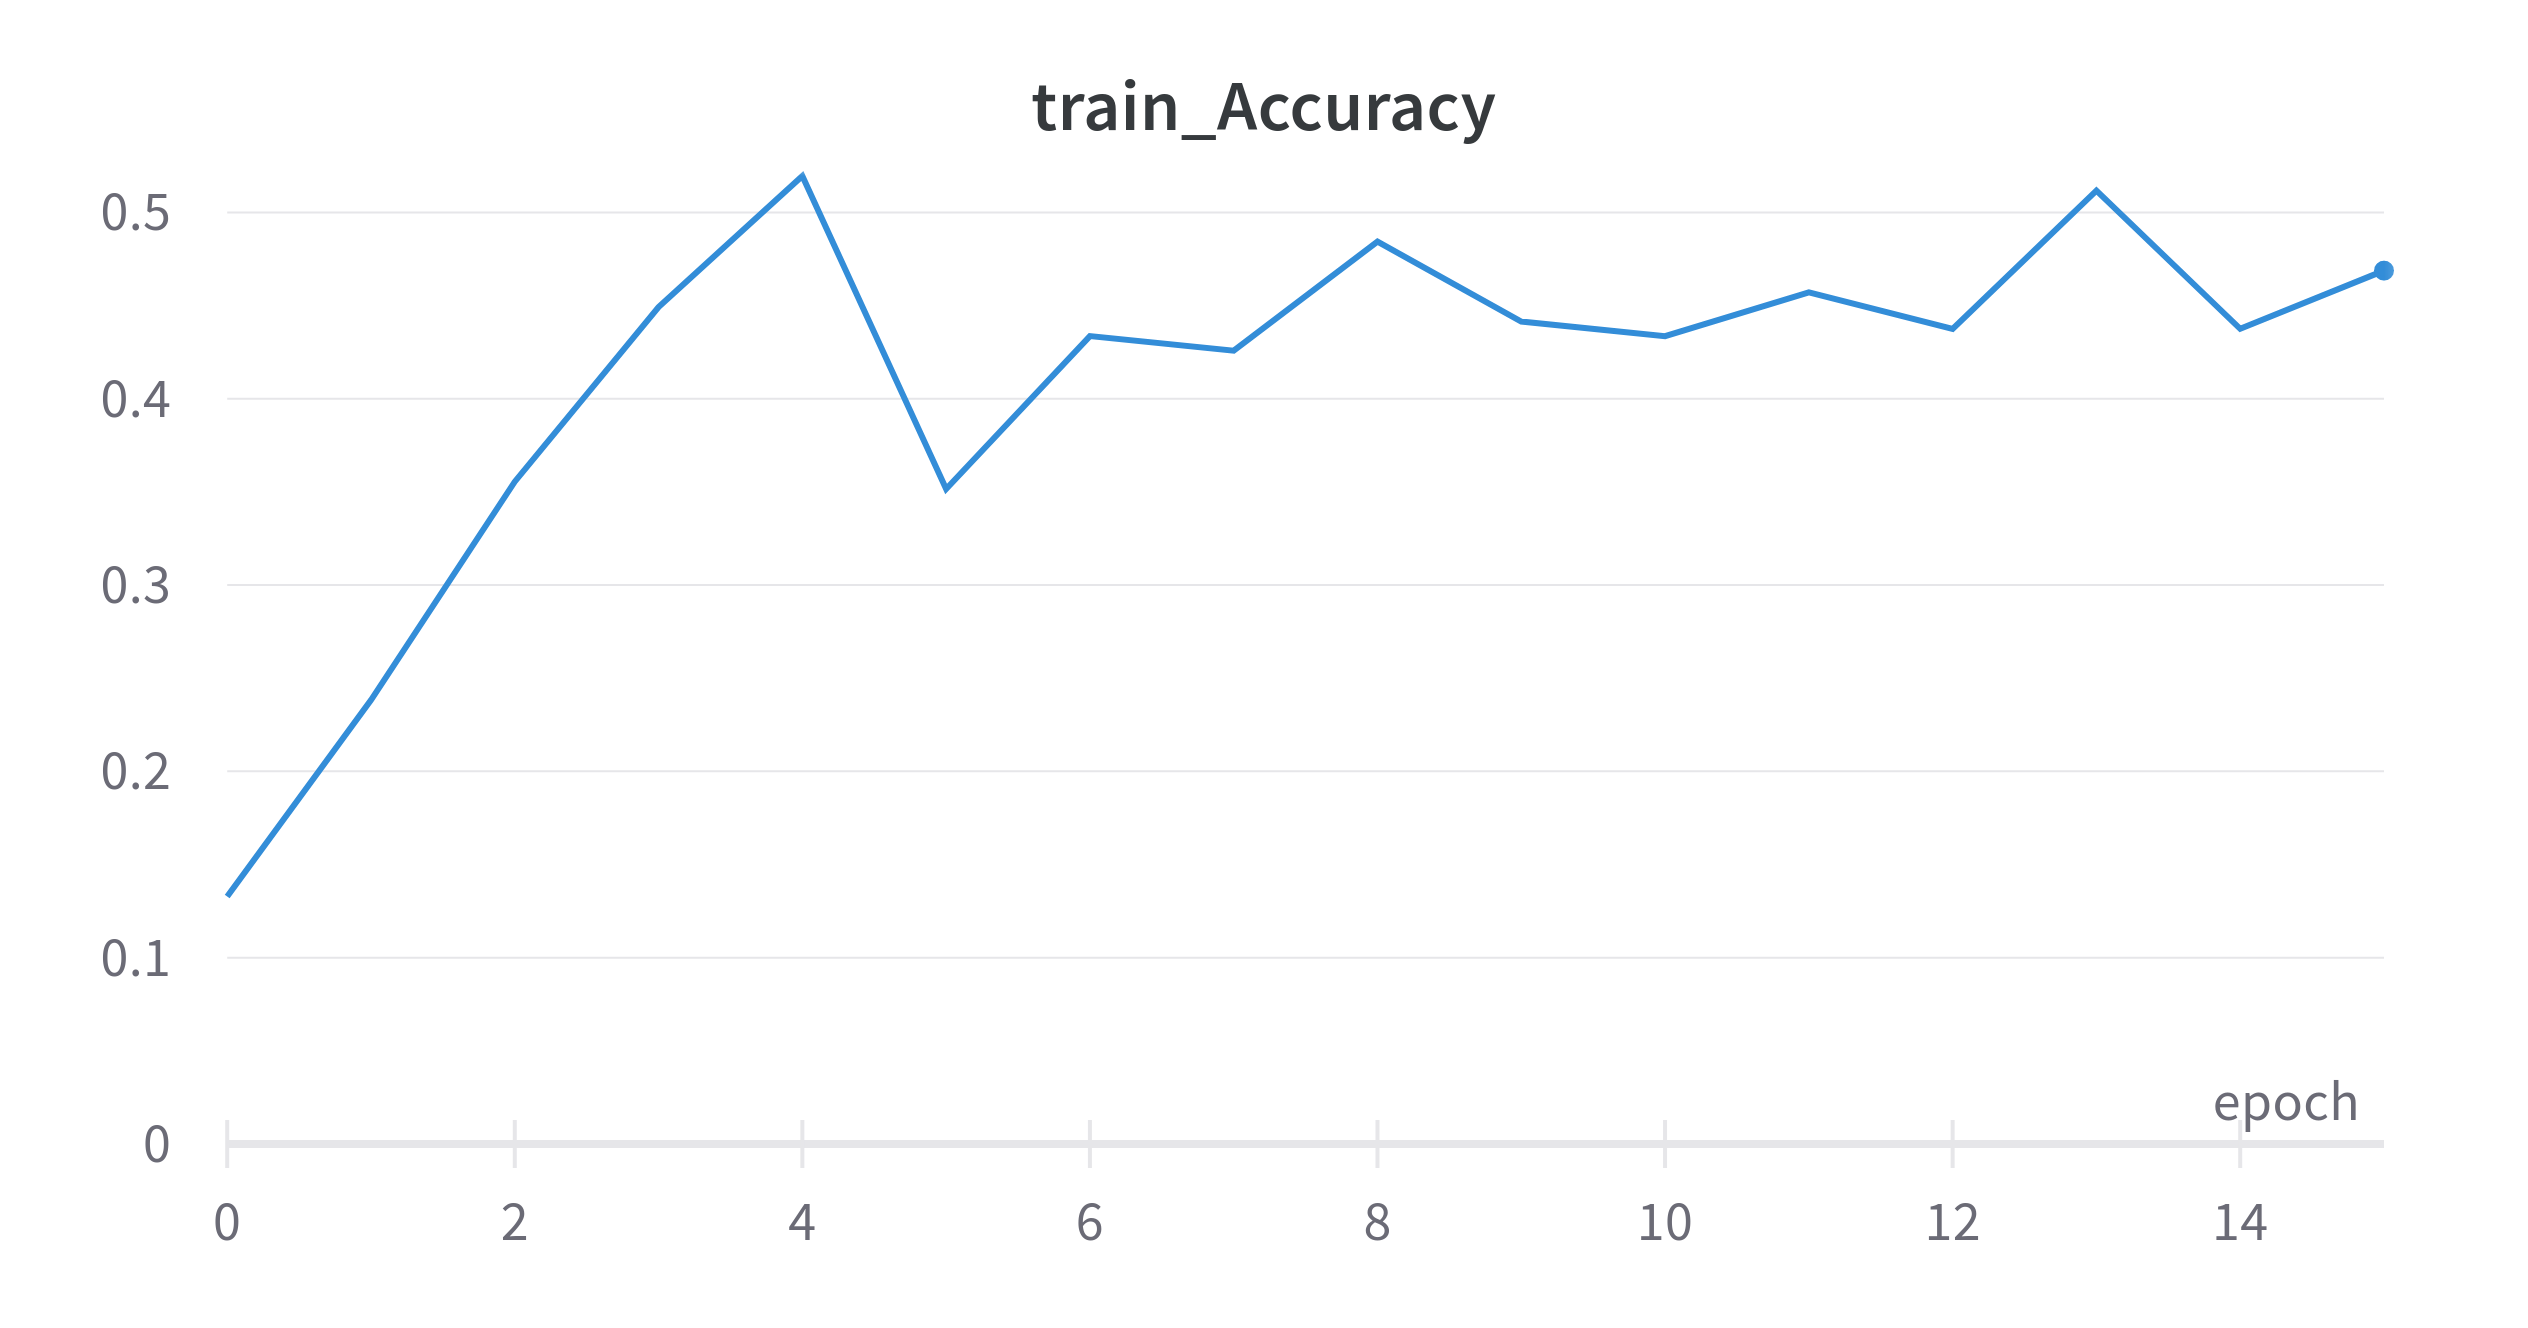
\includegraphics[width=.8\textwidth]{mnet_small_cifar10_accuracy_stride2.png}
	\caption{Cifar10 train accuracy using MobileNetV3 small and stride 2}
	\label{fig:cifar10_small_stride2_acc}
\end{figure}

\begin{figure}[H]
	\centering
	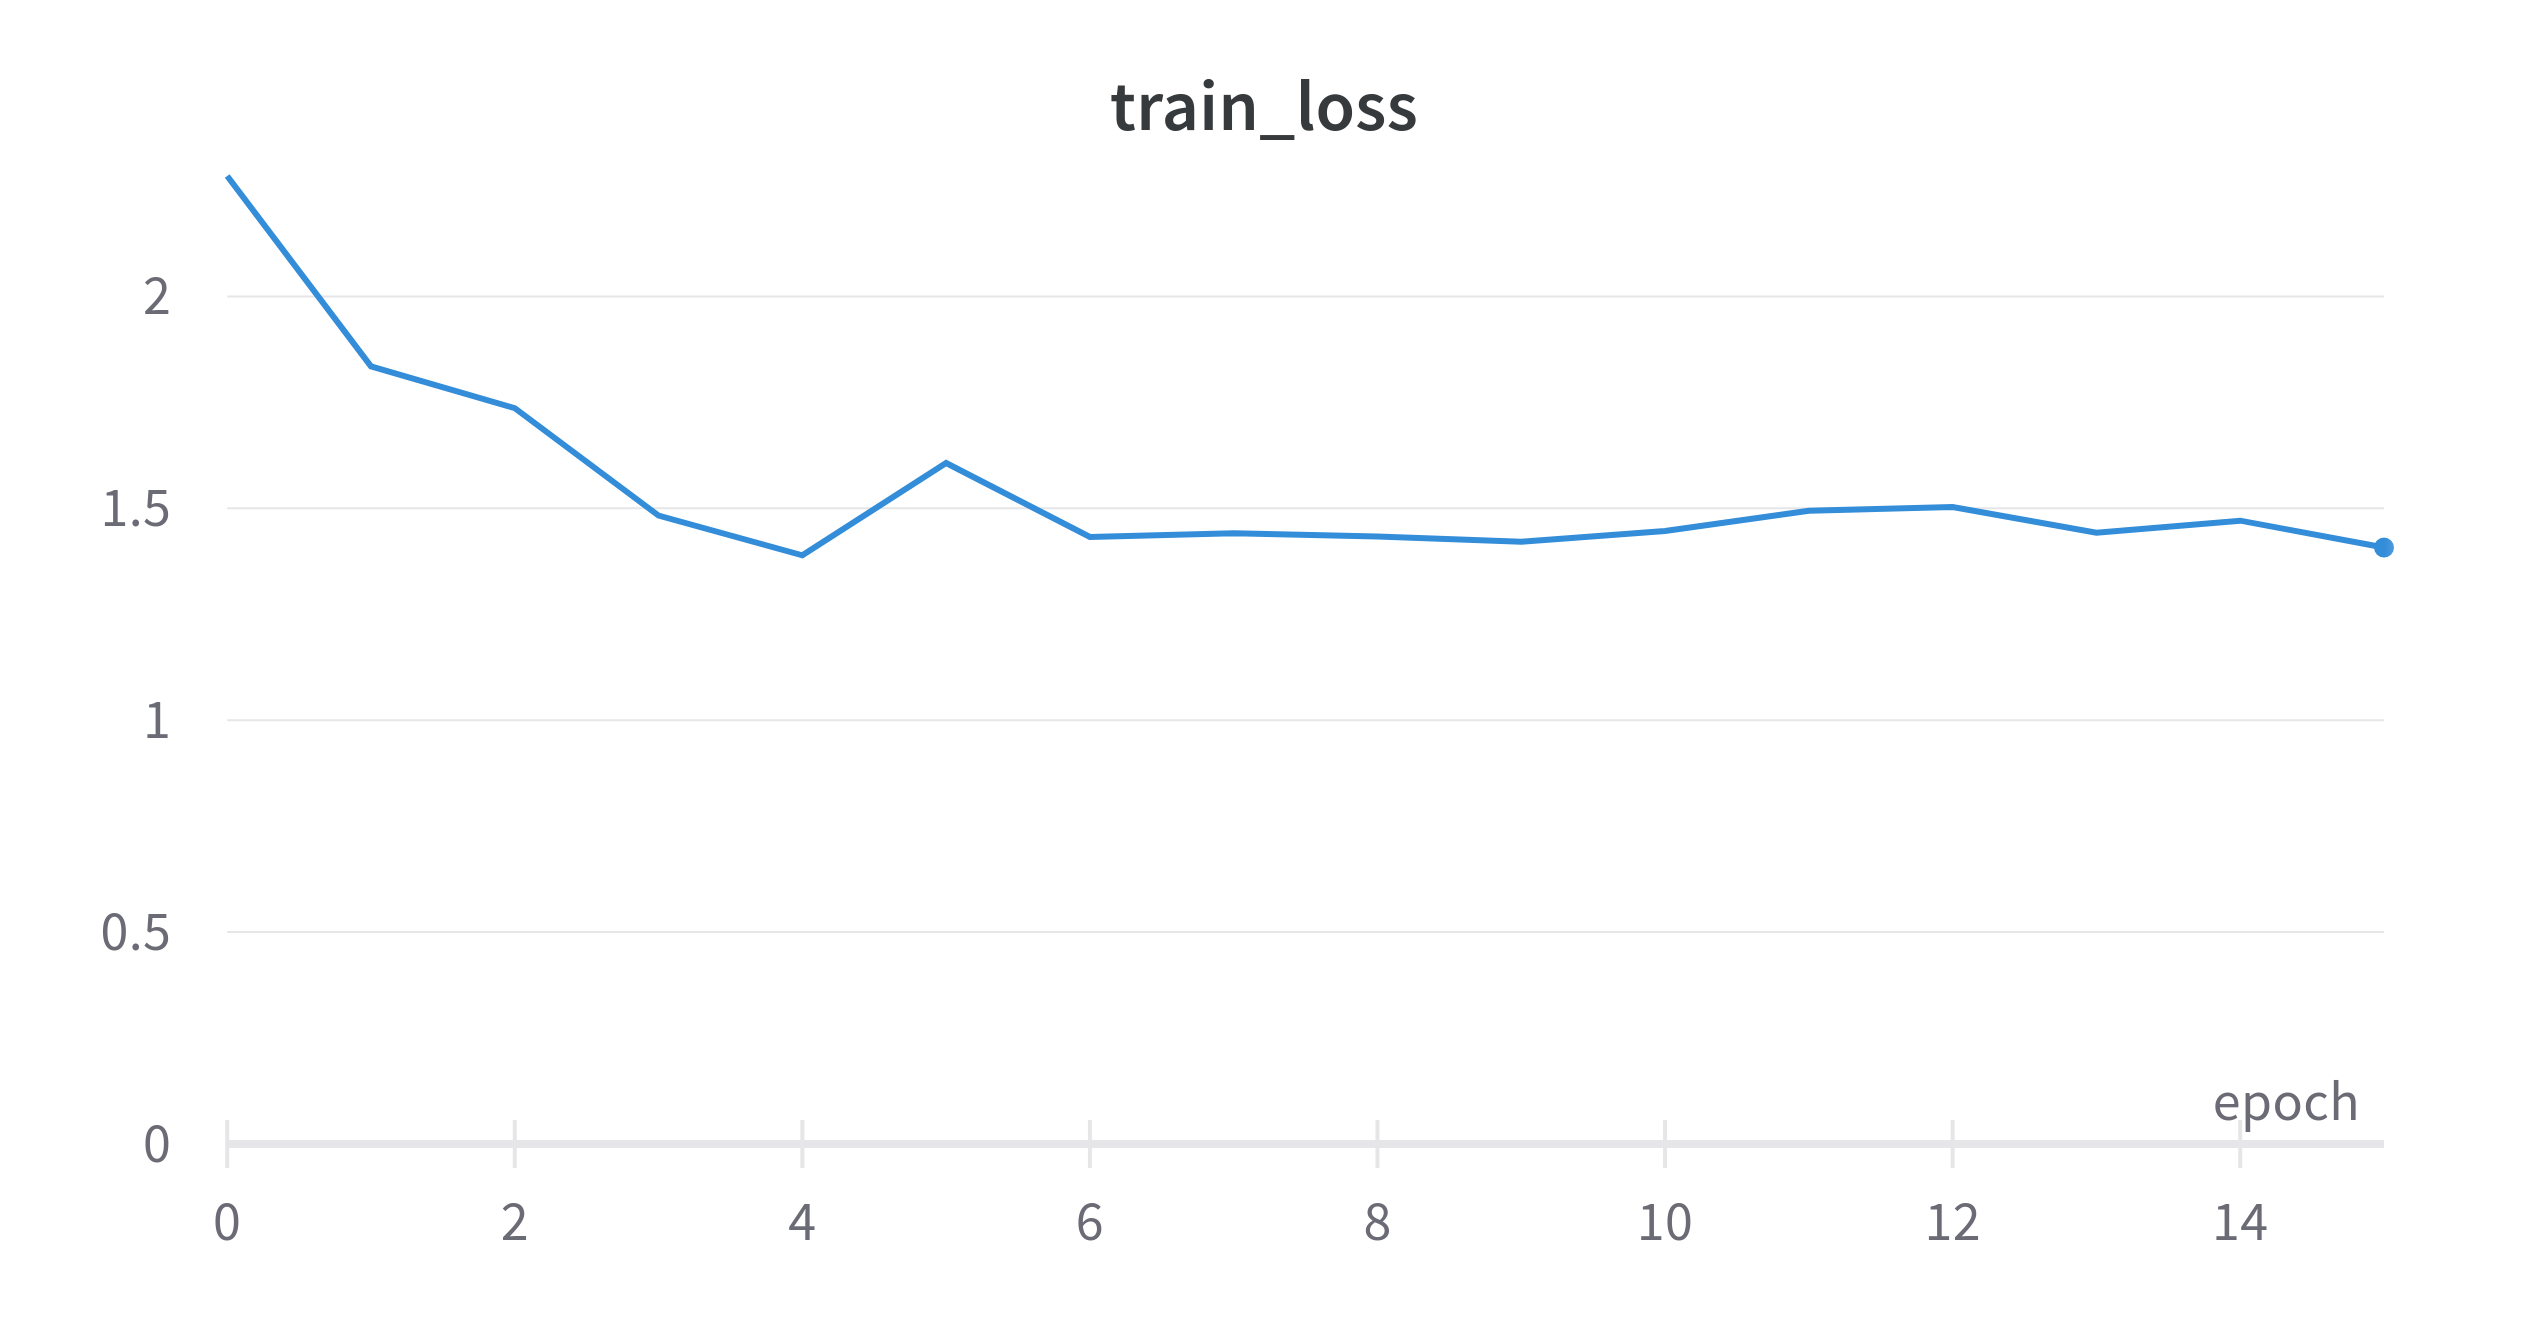
\includegraphics[width=.8\textwidth]{mnet_small_cifar10_loss_stride2.png}
	\caption{Cifar10 train loss using MobileNetV3 small and stride 2}
	\label{fig:cifar10_small_stride2_loss}
\end{figure}

This low training accuracy and loss is due to the datasets itself, it has very low image quality. An attempt to cut out this problem is done changing the stride of the first two convolutional layers. \\
In the architecture proposed by the authors, trained on the ImageNet dataset, the stride is set to two, loosing some informations in the convolution operation. For this type of dataset the stride is changed to one resulting in less information loss and better results. \\
In fact, as we can see from Figure~\ref{fig:cifar10_small_stride1_acc} and \ref{fig:cifar10_small_stride1_loss} the loss and accuracy gets better during training with this small change.

\begin{figure}[H]
	\centering
	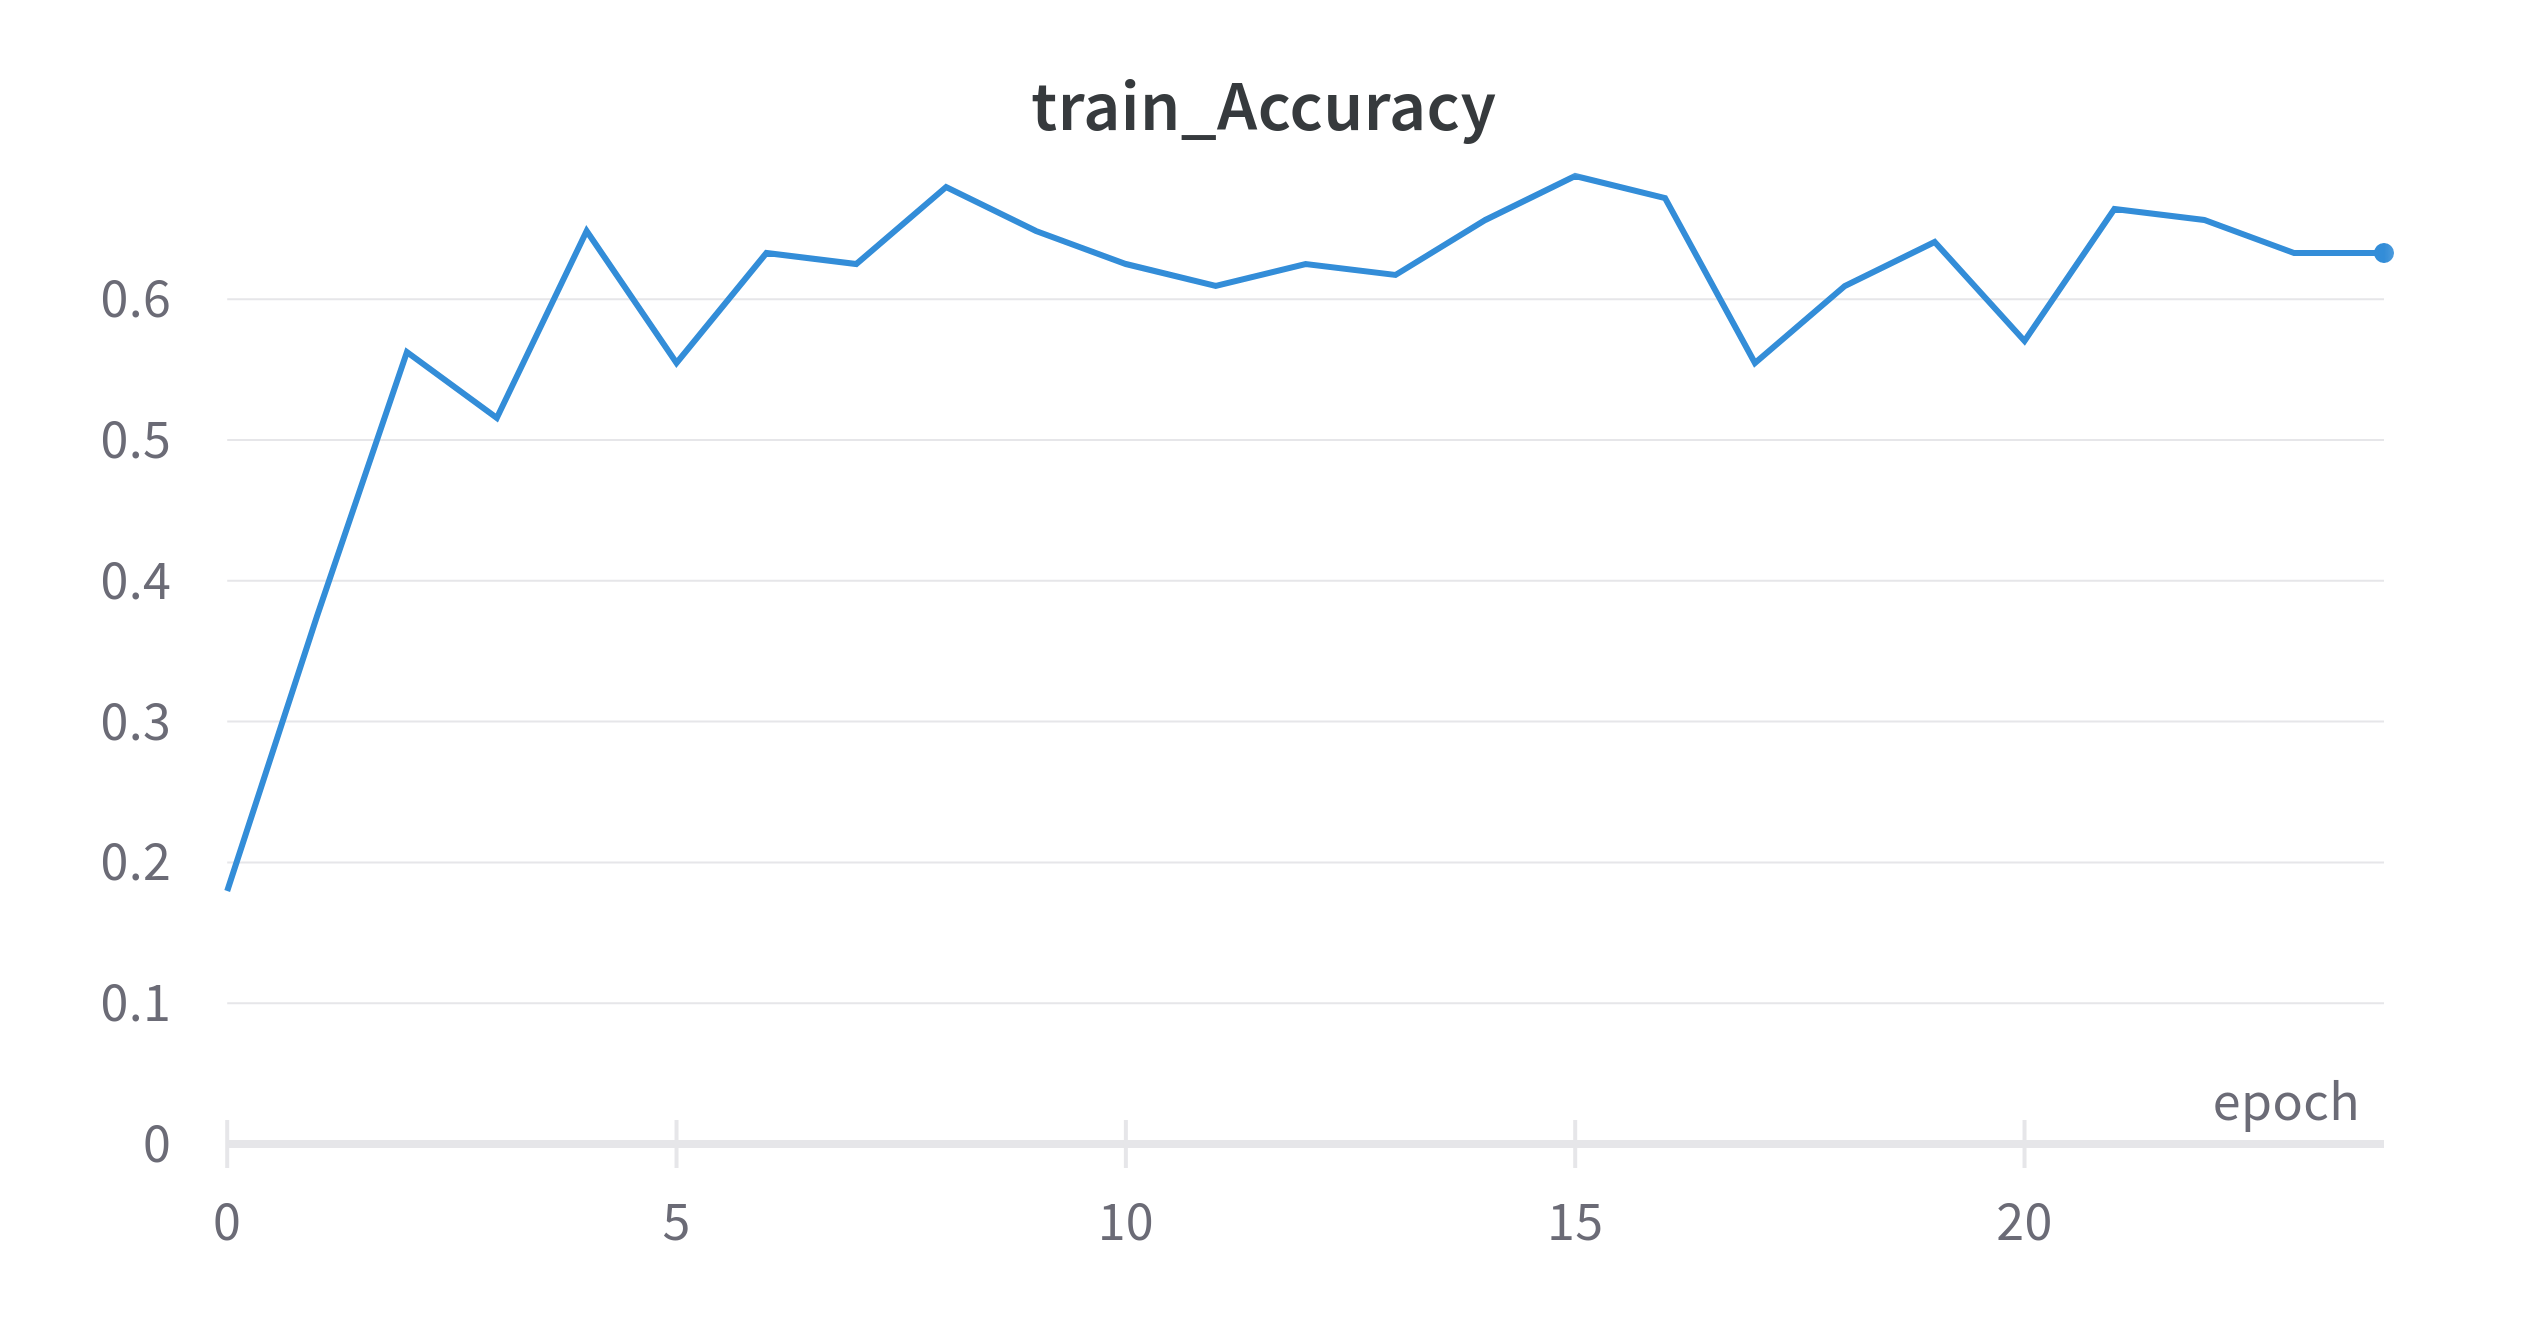
\includegraphics[width=.8\textwidth]{mnet_small_cifar10_accuracy.png}
	\caption{Cifar10 train accuracy using MobileNetV3 small and stride 1}
	\label{fig:cifar10_small_stride1_acc}
\end{figure}

\begin{figure}[H]
	\centering
	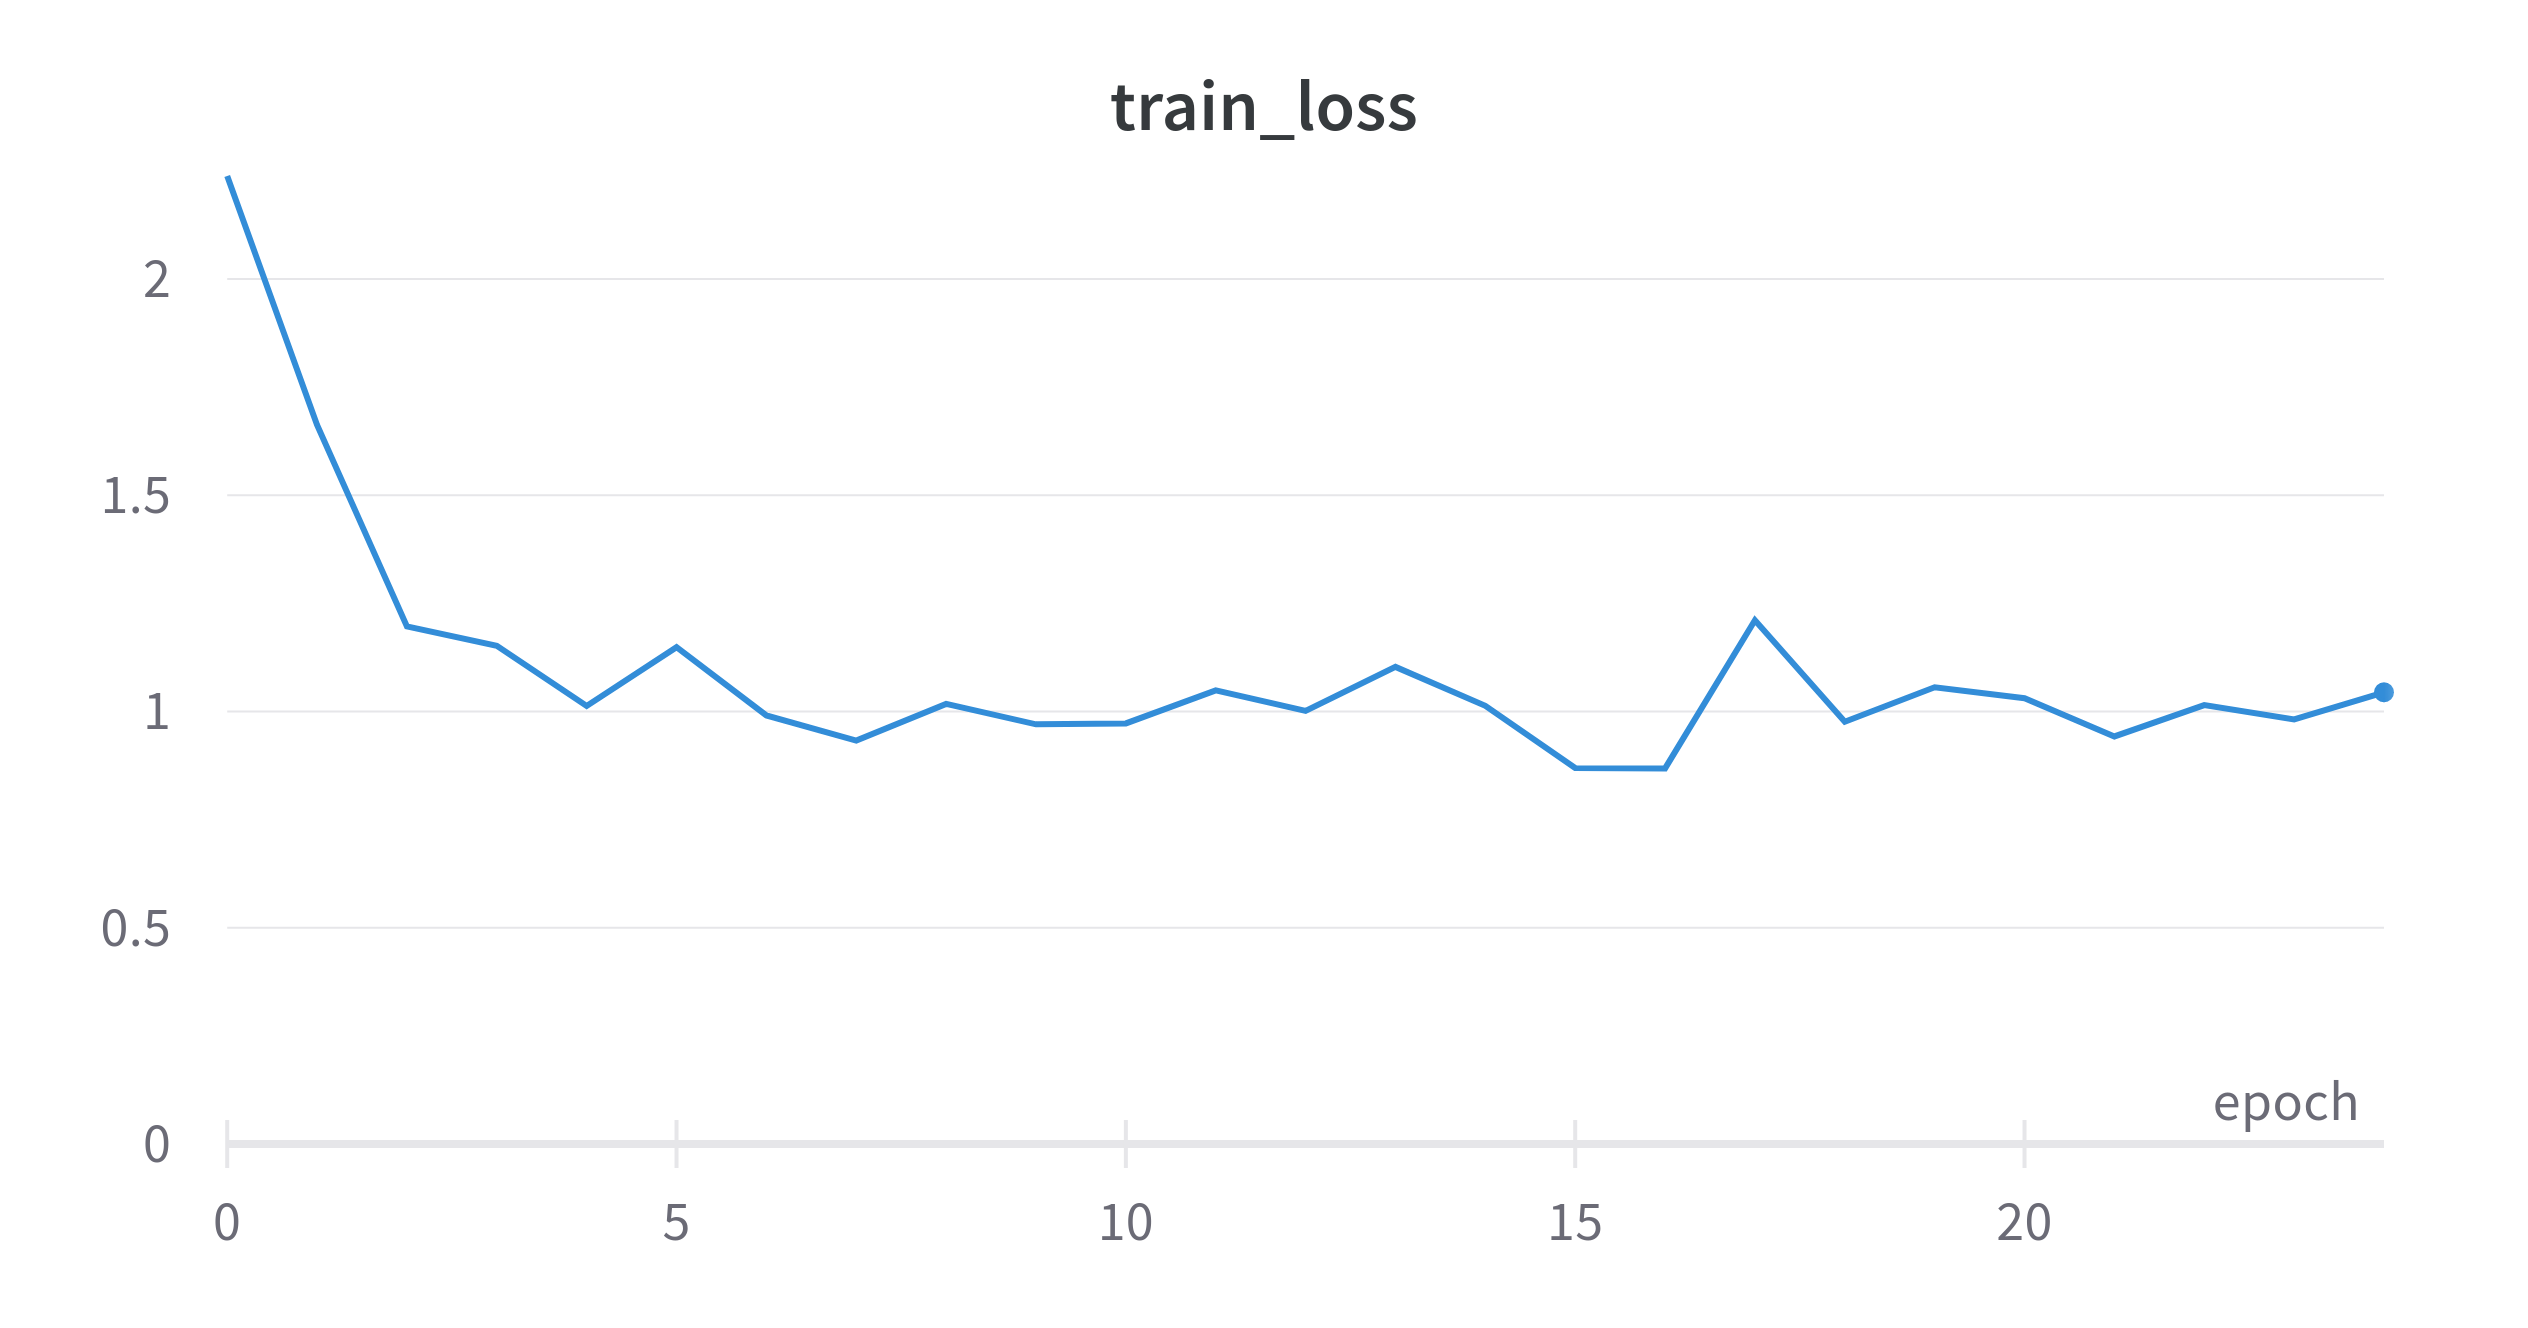
\includegraphics[width=.8\textwidth]{mnet_small_cifar10_loss.png}
	\caption{Cifar10 train loss using MobileNetV3 small and stride 1}
	\label{fig:cifar10_small_stride1_loss}
\end{figure}

As before, after training the test dataset is used for evaluation. In this case we notice an overall test accuracy very high, about $0.59\%$. The associated classification report with all the evaluation metrics is shown in Figure~\ref{fig:cifar10_small_stride1_report}.\\

In the confusion matrix plotted in Figure~\ref{fig:cifar10_small_stride1_cm} we can notice that the netwrok has low sensitivity with the class associated to label $2,3,4$ associated respectively to cat, deer and dog images. The network, therefore, is often confused in the identification of images belonging to these classes.

\begin{figure}[H]
	\centering
	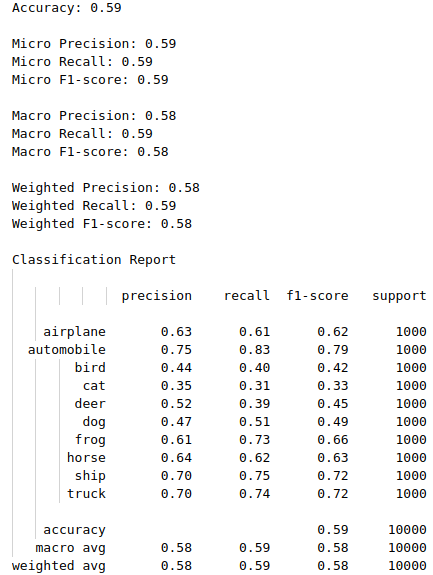
\includegraphics[width=.5\textwidth]{report_cifar10_small_stride1.png}
	\caption{Cifar10 classification report using MobileNetV3 Small and stride 1}
	\label{fig:cifar10_small_stride1_report}
\end{figure}

\begin{figure}[H]
	\centering
	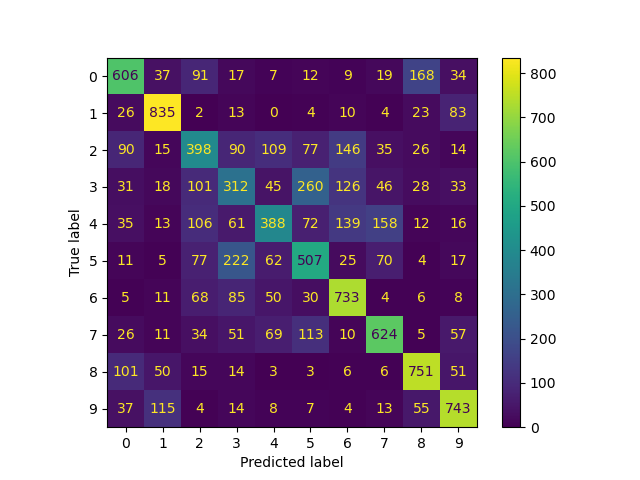
\includegraphics[width=.8\textwidth]{cm_cifar10_small_s1.png}
	\caption{Cifar10 confusion matrix using MobileNetV3 Small and stride 1}
	\label{fig:cifar10_small_stride1_cm}
\end{figure}

\paragraph{Large} 
Similarly to the Small version of MobileNetV3, the dataset is used to train MobileNet Large. \\
This time




\clearpage
\section{Conclusion}


\clearpage

\nocite{*}
\printbibliography[heading=bibintoc,title={References}]
\end{document}